\documentclass[xcolor={dvipsnames},pdf, hyperref={colorlinks=true, citecolor=ForestGreen, linkcolor=BlueViolet, urlcolor=Magenta}]{beamer}
\usetheme{Frankfurt}  
\usecolortheme{whale}
\usepackage{tikz} 
\usepackage{amsmath}
\usepackage{amsthm}
\usepackage{amssymb}              % used for \eqref{} in this document
\usepackage{dsfont}
\usepackage{hyperref}
\usepackage{threeparttable}
\usepackage{multirow}
\graphicspath{{Figures/}}
\usepackage{booktabs}
\usepackage{tikz}
\newtheorem{exmp}{Example}[section]
\usepackage{subcaption}
\usepackage{adjustbox}
\usepackage{graphicx}
\usepackage[mathscr]{euscript}
\usepackage{remreset}% tiny package containing just the \@removefromreset command
\makeatletter
\@removefromreset{subsection}{section}
\makeatother
\setcounter{subsection}{1}
\usepackage{float}
\usepackage{sgamevar}
\usepackage{sgame}
\theoremstyle{definition}

\newcommand{\defn}[1]{\textbf{#1}}


%Instructor version
\newcommand{\blank}[0]{}
\newcommand{\ddp}[1]{{\textcolor{ForestGreen}{#1}}} 
\newcommand{\dd}[1]{{\underline{\textcolor{ForestGreen}{#1}}}}

%Student version
%\newcommand{\blank}[0]{\vspace{2em}}
%\newcommand{\dd}[1]{\underline{\hspace{3cm}}} 
%\newcommand{\ddp}[1]{}

\addtobeamertemplate{navigation symbols}{}{%
	\usebeamerfont{footline}%
	\usebeamercolor[fg]{footline}%
	\hspace{1em}%
	\insertframenumber/\inserttotalframenumber
}

%% preamble
\title{Supply and Demand}
\author{David A. D\'iaz}
\institute{UNC Chapel Hill}
\date{}

\AtBeginSection[] %Section links on slides

\section{Demand}

\begin{document} 
	
	\begin{frame}
		
		\titlepage
		
	\end{frame}
	
\begin{frame}{Markets and Competition}
	\begin{itemize}
		\item \defn{Market:} A group of buyers and sellers of a particular good or service.
		
		\item \defn{Competitive Market:} A market in which there are many buyers and many sellers so that each has negligible impact on the market price.
		
		\item For the next few chapters, we will focus on markets that are \textbf{perfectly competitive.} 
		\begin{itemize}
			\item Goods are exactly the same 
			\item Buyers \& sellers are price takers 
		\end{itemize}
		\item Other types of markets: monopolies, oligopolies. We will study those later.
	\end{itemize}
\end{frame}

\begin{frame}{Demand}
	
	\begin{itemize}
		\item \defn{Quantity Demanded:} The amount of a good or service that buyers are willing and able to purchase.
		
		\begin{exmp}
			\small
			Table \ref{tab11} below shows how many used economics textbooks students in this class are willing to buy at different prices.
			\begin{table}[ht]
				\caption{David's Class}
				\label{tab11}
				\centering
				\begin{tabular}{  c| c}        
					
					Price   & Quantity Demanded \\
					\hline
					\$60 & 0 \\
					\$50 & 3 \\
					\$40 & 6 \\
					\$30 & 9 \\
					\$20& 12 \\
					\$10 & 15 \\
					\$0 & 18 \\
				\end{tabular}
			\end{table} 
			
			This kind of table is referred to as a \dd{demand schedule}.
		\end{exmp}
	\end{itemize}


\end{frame}


\begin{frame}[b]{Demand}
	

	\begin{figure}[H]
		\centering
		\ddp{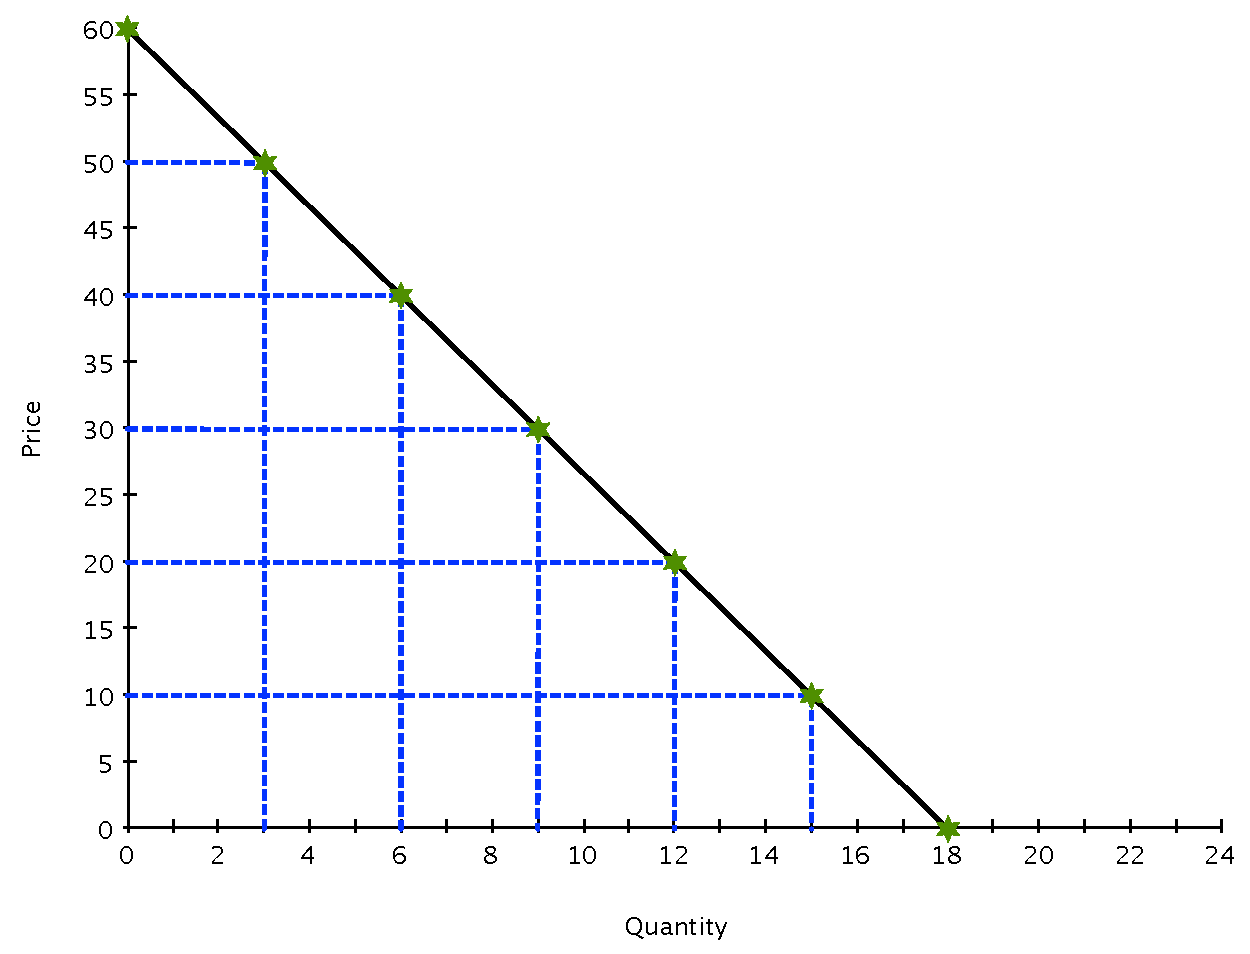
\includegraphics[scale=.30]{plot7.pdf}}
		\caption{Demand for Textbooks}
	\end{figure}
\end{frame}


\begin{frame}{Demand}
\begin{itemize}
	\item Notice that by convention, we plot \dd{prices} on the y-axis and \dd{quantity} on the x-axis.
	\item Both the table and the curve demonstrate the \defn{Law of Demand:} All else equal, the quantity demanded of a good increases when the price of the good decreases.
\end{itemize}
\end{frame}

\begin{frame}{Demand}
		\begin{exmp} 
			\scriptsize	
				Suppose student's in Wenting's Econ 101 class are willing to buy used textbooks according to Table \ref{tab2}.
				
				\begin{table}[ht]
					\caption{Wenting's Class}
					\label{tab2}
					\centering
					\begin{tabular}{  c|c}        
						
						Price   & Quantity Demanded \\
						\hline
						\$60 & 2 \\
						\$50 & 4 \\
						\$40 & 6 \\
						\$30 &  8 \\
						\$20& 10 \\
						\$10 & 12 \\
						\$0 & 14 \\
					\end{tabular}
				\end{table} 
				
			\begin{enumerate}
			\item 	If these two classes make up the market for used economics textbooks at UNC, what is the market quantity demanded at each price? Draw the market demand curve.
	
			\item 	If the price of used economics textbooks is \$40, how many books will be demanded? What if the price increased to \$50? 
			\end{enumerate}
			\end{exmp}
		
	
		
	\end{frame}


\begin{frame}[b]{Demand}
		\begin{figure}[H]
			\centering
			\ddp{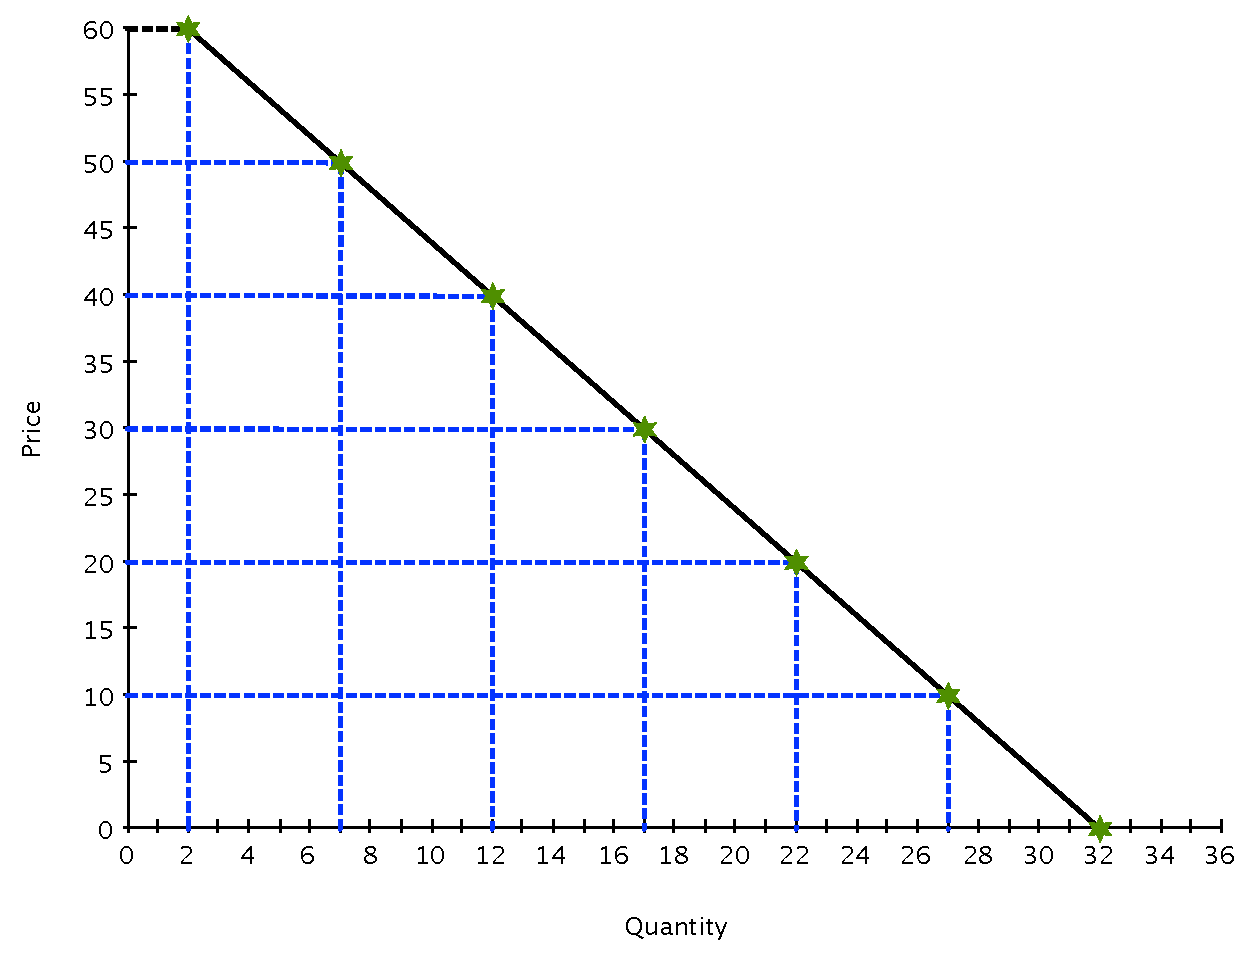
\includegraphics[scale=.30]{plot8.pdf}}
			\caption{Demand for Textbooks}
		\end{figure}
	\end{frame}

\begin{frame}{Demand}
	\begin{itemize}
	\item Notice that a change in price caused \dd{a movement along the demand curve}.
	\item This is referred to as a \dd{change in quantity demanded}.
\end{itemize}
\end{frame}
	
\begin{frame}{Demand}
		\begin{itemize}
			\item The demand curve holds everything but price and quantity demanded constant. 
			\item But there are other things that affect how much people are willing to purchase at any given price. 
			\item Changes in these factors cause \dd{shifts} of the demand curve. 
			\item This is referred to as a \dd{change in demand}.
		\end{itemize}
\end{frame}


	\begin{frame}{Demand}
	\begin{itemize}
		\item Increase in demand (shift right): 
		\begin{itemize}	
			\item Horizontal reading: At any given price, willing and able to purchase more. 
			\item Vertical: At any given quantity, willing and able to pay more. 
		\end{itemize}
	\end{itemize}
\blank 
\blank 
\blank 
\blank
	\begin{figure}
		\ddp{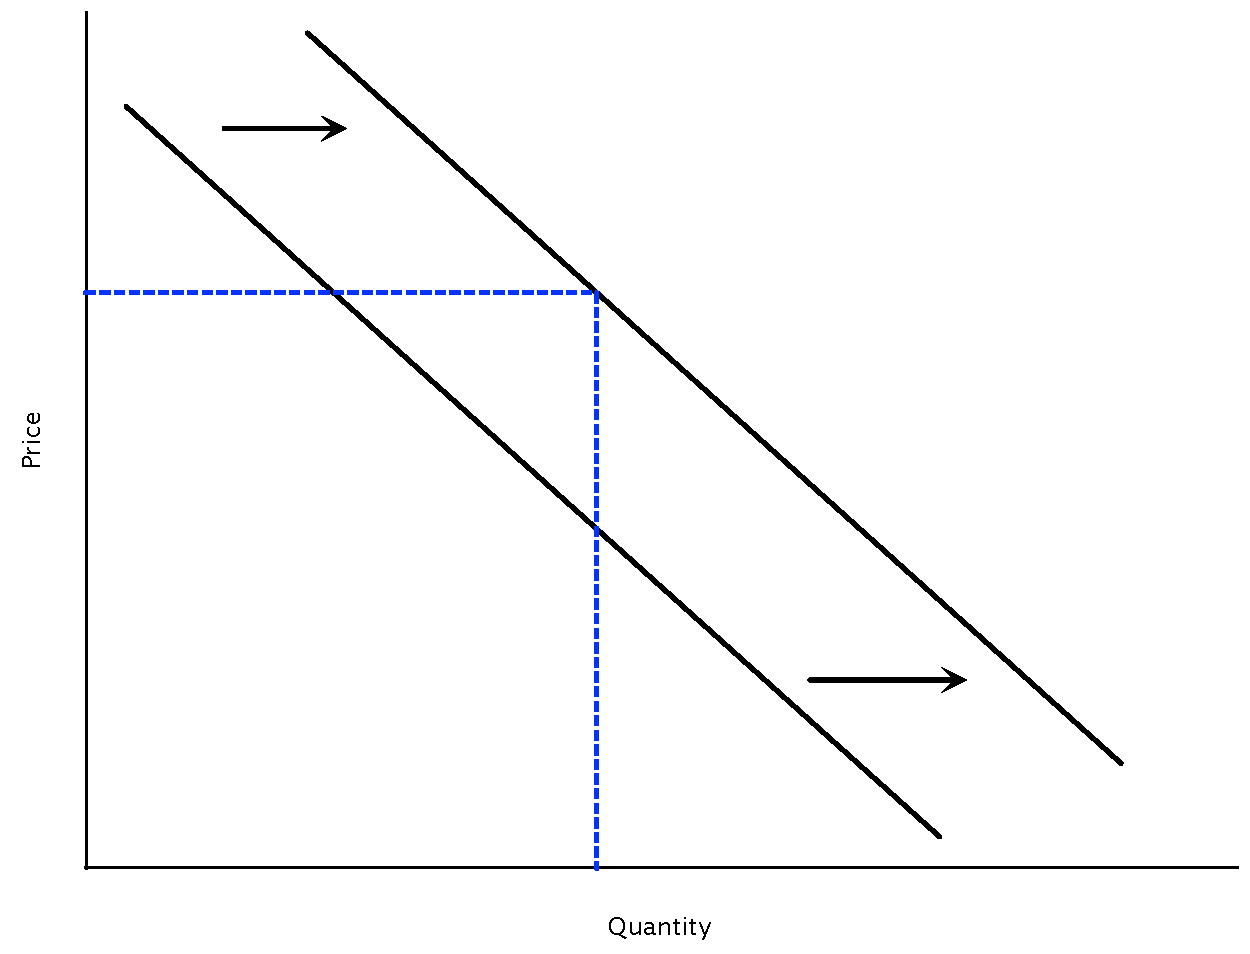
\includegraphics[scale=.25]{plot9.pdf}}
		\caption{Increase in Demand}
	\end{figure}
	
\end{frame}
	
\begin{frame}[b]{Demand}
	\begin{itemize}
	\item Decrease in demand (shift left):
\begin{itemize} 
	\item Horizontal reading: At any given price, willing and able to purchase less.
	\item Vertical: At any given quantity, willing and able to pay less. 
\end{itemize}
	\end{itemize}
	\blank 
	\blank 
	\blank 
	\blank
			\begin{figure}
				\centering
				\ddp{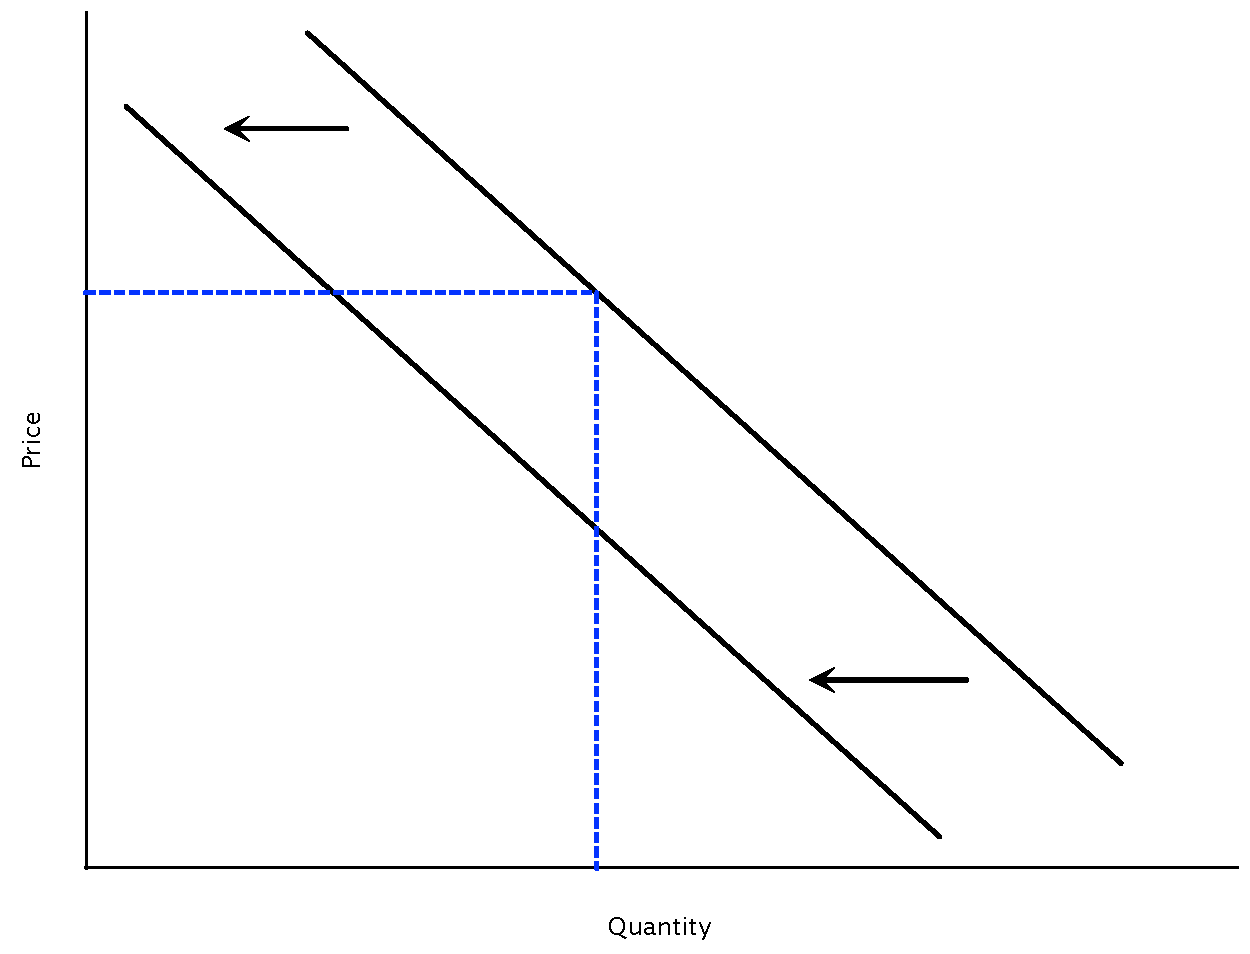
\includegraphics[scale=.25]{plot10.pdf}}
				\caption{Decrease in Demand}
			\end{figure}
\end{frame}

	
	
\begin{frame}{Demand}
	\textbf{Variables that Shift the Demand Curve}
			\begin{enumerate}
				\item Income

			
			\begin{itemize}
				\item \defn{Normal good:} A good for which an increase in income leads to an \dd{increase} in demand. This describes most goods.
				\item \defn{Inferior good:} A good for which an increase in income leads to a \dd{decrease} in demand (e.g., ramen soup).
			\end{itemize}

			\item Prices of related goods
		\begin{itemize}
			\item \defn{Substitutes:} Goods for which an increase in the price of one leads to an \dd{increase} in demand for the other.
			\item \defn{Complements:} Goods for which an increase in the price of one leads to a \dd{decrease} in demand for the other.
		\end{itemize}
	
		\end{enumerate}
\end{frame}

	
\begin{frame}{Demand}
		\textbf{Variables that Shift the Demand Curve}
	\begin{enumerate}
		\setcounter{enumi}{2}	
		\item Tastes: The perception of products affects how in-demand they are. News, cultural changes, etc. will change preferences.
		\item Expectations: Expected future prices affect current demand. If prices are predicted to increase in the future, then demand today will \dd{increase}. If prices are predicted to decrease, demand today will \dd{decrease}.
		\item Number of buyers: More buyers $\Rightarrow$ \dd{greater} demand.
	\end{enumerate}
\end{frame}

\begin{frame}[t]{Demand}
	\begin{exmp}
		\small
		Consider the demand for cigarettes. What happens to demand in each of the following scenarios? Explain why.
		\begin{enumerate}
			\item	The surgeon general declares that cigarettes are even more harmful than previously believed.
			

			\item	Individuals start believing a rumor that the government is going to raise the cigarette tax by \$1.00.
			
		
			
			\item 	The price of beer increases (assume cigarettes and beer are complements.). 
			
			
			
			\item The price of cigarettes decreases.  
			
		\end{enumerate}
	\end{exmp}


\ddp{\pause \small (1) Demand decreases due to a change in tastes \\
\pause (2) Demand today will increase because the EFP increased \\
\pause (3) Demand decreases due to increase in price of complement \\
\pause (4) Demand doesn't shift. Quantity demanded will increase}
\end{frame}



	
\begin{frame}{Demand}
	\begin{itemize}
		\item To reiterate:
		\begin{itemize}
			\item Changes in the price of a good will affect the quantity demanded and cause a movement along a given demand curve
			\item Changes in the variables discussed above affect each individual's willingness to pay and cause a shift of the entire demand curve
		\end{itemize}
	\end{itemize}
\end{frame}

\section{Supply}

\begin{frame}{Supply}
	
\begin{itemize}
	\item 	\defn{Quantity Supplied:} The amount of a good that sellers are able and willing to sell.
	
	\item \defn{Law of Supply:} All else equal, the quantity supplied of a good rises when the price of the good rises.
	
	\item \defn{Supply Schedule:} A table that shows the relationship between the price of a good and the quantity supplied.
	
	\item \defn{Supply Curve:} A graph that shows the relationship between the price of a good and the quantity supplied, holding constant everything else that influences how much sellers of the good want to sell.
	
	\item \defn{Market Supply:} The sum of all the individual supplies for a particular good or service.
\end{itemize}
		
\end{frame}

\begin{frame}{Supply}
	
\begin{itemize}
	\item Just like the demand curve, the supply curve holds everything but price and quantity constant. 
	\item If the price of a good changes, that will lead to a \dd{movement along the supply curve}.
	\item But there are other things that affect how much sellers are willing to sell at any given price. 
	\item Changes in these factors cause shifts of the supply curve. Similar to demand, this is referred to as a \dd{change in supply}. 
\end{itemize}
	
\end{frame}

\begin{frame}[b]{Supply}
		\begin{itemize}
		\item Increase in supply (shift right): 
		\begin{itemize} 
			\item Horizontal: At any given price, willing and able to sell more of a good.
			\item Vertical: At any given quantity, willing to sell good for a lower price. 
		\end{itemize}
	\end{itemize}
\blank 
\blank 
\blank 
\blank
\begin{figure}[H]
		\ddp{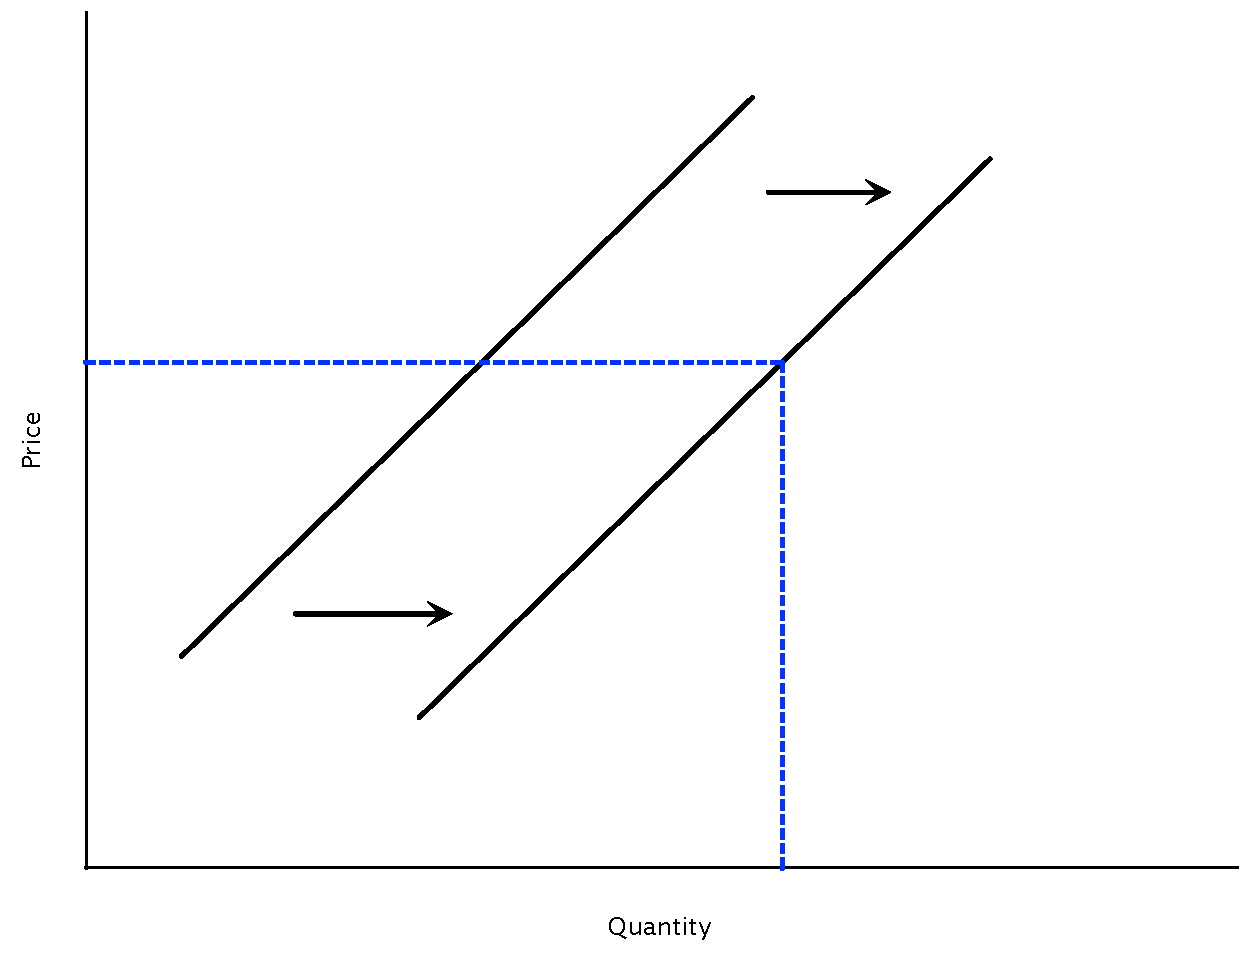
\includegraphics[scale=.30]{plot11.pdf}}
		\caption{Increase in Supply}
	\end{figure}

\end{frame}
\begin{frame}{Supply}
	
	\begin{itemize}
		\item Decrease in supply (shift left): 
		\begin{itemize}
			\item Horizontal: At any given price, willing and able to sell less of a good.
			\item Vertical: At any given quantity, willing to sell good for a higher price. 
		\end{itemize}
	\end{itemize}
\blank 
\blank 
\blank 
\blank
	\begin{figure}
	\centering
	\ddp{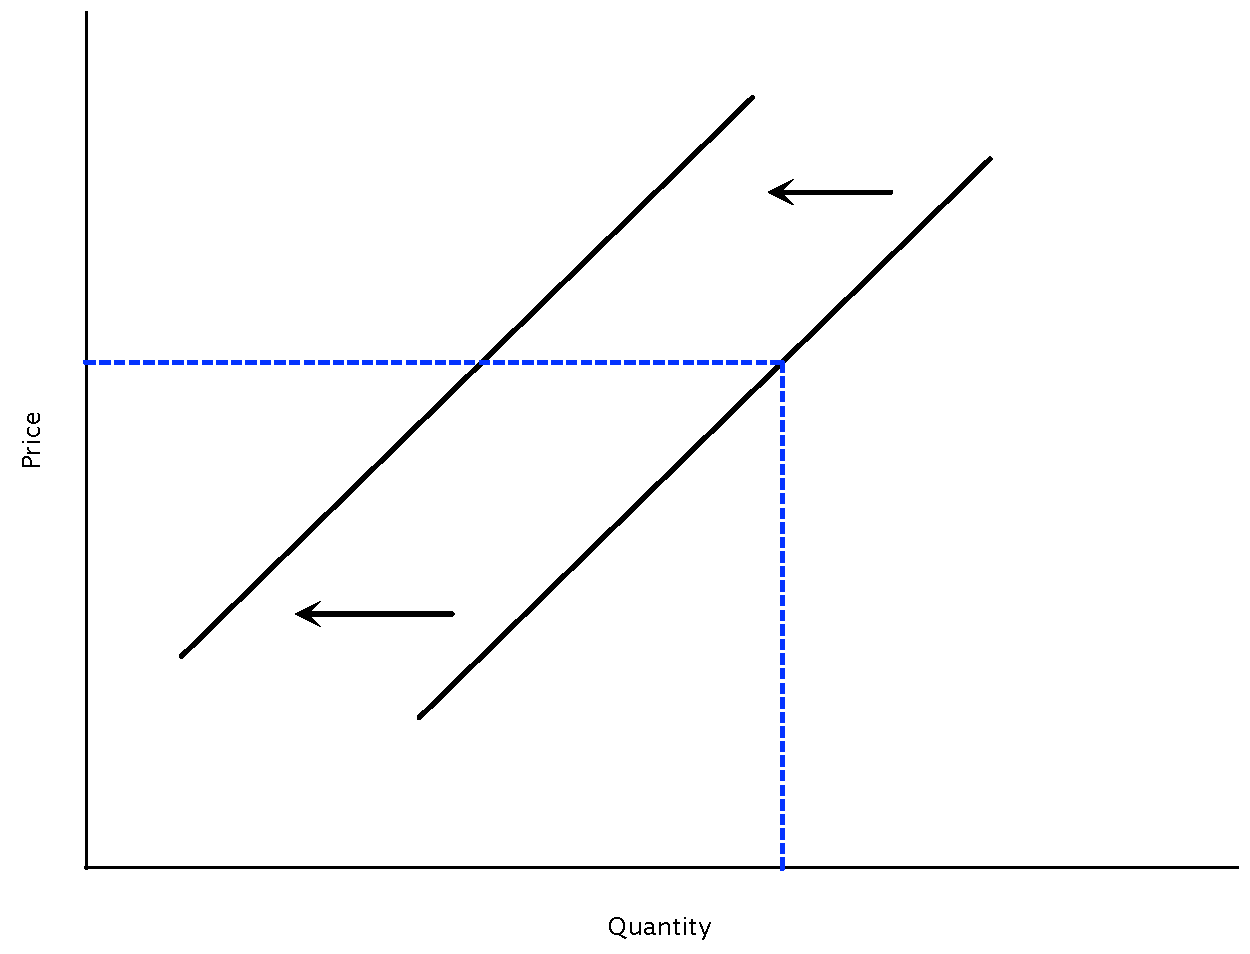
\includegraphics[scale=.30]{plot12.pdf}}
	\caption{Decrease in Supply}
\end{figure}
	
\end{frame}

\begin{frame}{Supply}
	\textbf{Variables that Shift the Supply Curve}
		\begin{enumerate}
			\item Input prices 
			\begin{itemize}
				\item Higher input prices mean that suppliers must receive a higher price to sell any given quantity. Supply will \dd{decrease}.
				\item Lower input prices imply sellers are willing to accept less to supply a given quantity. Supply will \dd{increase}.
			\end{itemize}  
			\item Technology 
			\begin{itemize}
				\item Advances in technology lower costs of production and thus allow firms to sell more for any given price. Supply will \dd{increase}. 
			\end{itemize}
		\end{enumerate}
\end{frame}

\begin{frame}{Supply}
	\textbf{Variables that Shift the Supply Curve}
	\begin{enumerate}
			\setcounter{enumi}{2}	
		\item Expectations
		\begin{itemize}
			\item If prices are expected to increase in the future, supply today will \dd{decrease}.
			\item If prices are expected to decrease in the future, supply today will \dd{increase}.
		\end{itemize} 
		\item Number of sellers 
		\begin{itemize}
			\item More sellers $\Rightarrow$ \dd{increase} in supply.
		\end{itemize}
	\end{enumerate}
\end{frame}

\begin{frame}[t]{Supply}
	\begin{exmp}
		Consider the supply for cigarettes.  What happens in each of the following scenarios? Explain why.
		
		\begin{enumerate}
			\item The minimum wage is increased.
		
			
			\item	A new device is invented that harvests tobacco at $1/2$ the previous cost.
			
			\item 	The price of cigarettes increases.
			

			
			\item	An overseas cigarette manufacturer starts producing in America.
		
		\end{enumerate}
	\end{exmp}

\ddp{\pause (1) Supply decreases due to an increase in an input price \\
\pause (2) Supply increases due to better technology\\
\pause (3) Movement along the curve. Quantity supplied increases \\
\pause (4) Supply increases because there are more sellers in the market}
\end{frame}

\section{Market Equilibrium}

\begin{frame}{Market Equilibrium}
	\begin{itemize}
		\item \textbf{Principle 6: Markets are Usually a Good Way to Organize Economic Activity}
		\item \defn{Equilibrium:} The point at which the market price is such that $Q_D = Q_S$.
		\item \defn{Equilibrium price:} The price that balances $Q_D$ and $Q_S$. Denoted $P^*$.
		\item \defn{Equilibrium quantity:} $Q_D$ and $Q_S$ at the equilibrium price. Denoted $Q^*$.
	\end{itemize}
\end{frame}

\begin{frame}[b]{Market Equilibrium}
		
		\begin{figure}[H]
			\centering
			\ddp{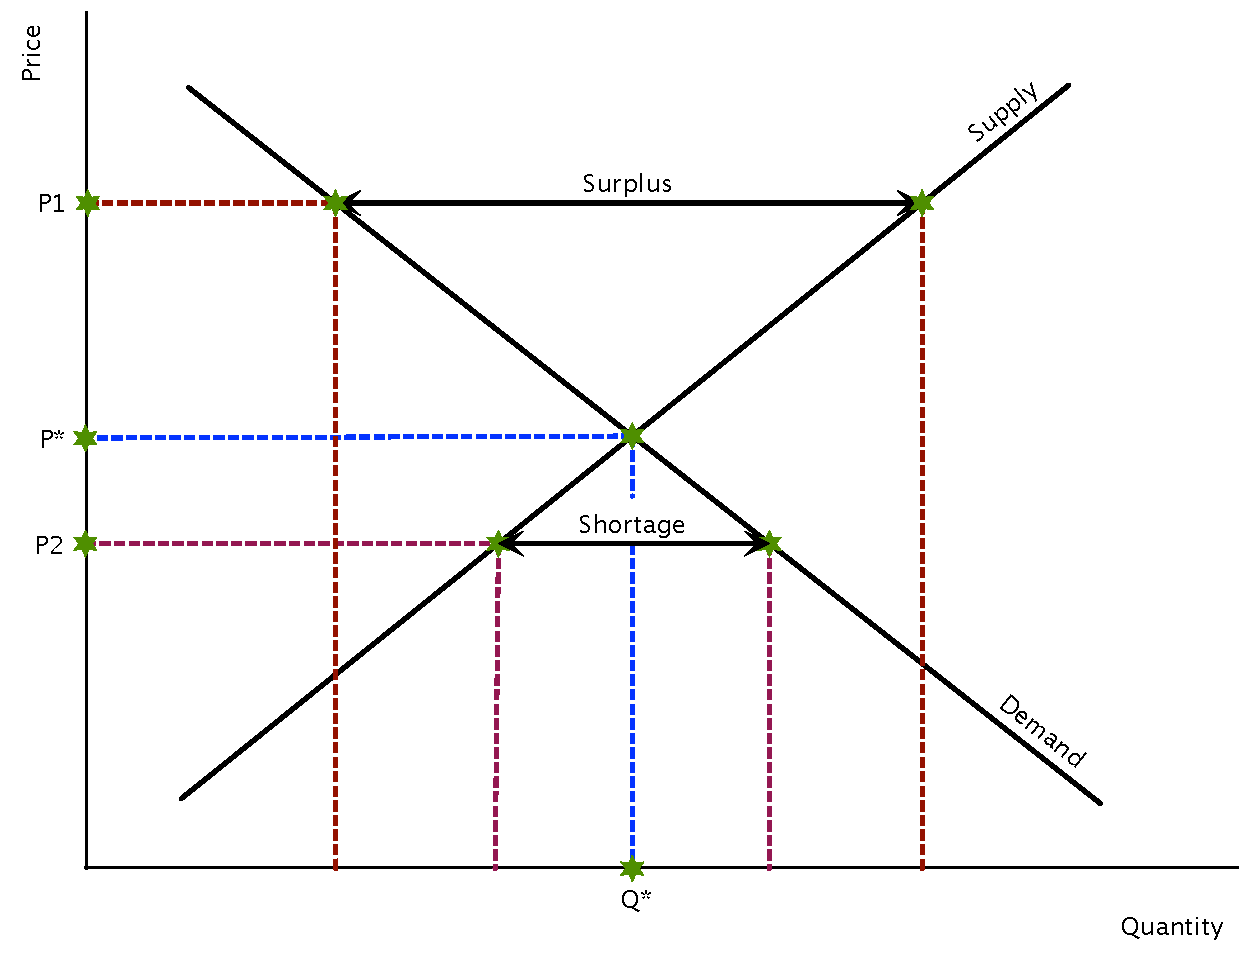
\includegraphics[scale=.4]{plot13.pdf}}
			\caption{Market Equilibrium}
		\end{figure}
		
	
\end{frame}

\begin{frame}{Market Equilibrium}
	\begin{itemize}
		\item	Graphically, the equilibrium is given by the point where the two curves intersect. $P^*$ and $Q^*$ denote the equilibrium price and quantity, respectively.
		\item 	What if the market price was $P_1>P^*$? 
		\begin{itemize}
			\item At this price, we  have that \dd{quantity supplied} is greater than \dd{quantity demanded}. 
			\item This is referred to as a \dd{surplus}. 
			\item There will be \dd{downward} pressure on prices. \item These changes in prices represent movements \textit{along} the supply and demand curves.
		\end{itemize}	
		
	\end{itemize}
\end{frame}

\begin{frame}{Market Equilibrium}
\begin{itemize}
\item What if the market price was $P_2<P^*$? 
\begin{itemize}
	\item At this price, we would have that \dd{quantity demanded} is greater than \dd{quantity supplied}.
	\item This is referred to as a \dd{shortage}. 
	\item  In this scenario, there is \dd{upward} pressure on prices. 
\end{itemize}
\end{itemize}
\end{frame}

\begin{frame}{Market Equilibrium}
	\begin{itemize}
		\item 	Importantly, no matter what the price is originally, the activities of the buyers and sellers automatically push the market price toward the equilibrium price.
		\item \defn{The Law of Supply and Demand:} The price of a good adjusts to bring the quantity demanded and quantity supplied for that good into balance. 
	\end{itemize}
\end{frame}


\begin{frame}{Market Equilibrium}
	\scriptsize
	\begin{exmp} A survey indicated that chocolate is Americans' favorite ice cream flavor. For each of the following, indicate the possible effects on demand, supply, or both as well as the effect on the equilibrium price and quantity of chocolate ice cream.
		\begin{enumerate}
			
			
			\item A severe drought in the Midwest causes dairy farmers to reduce the number of milk-producing cattle in their herds by a third. These farmers supply cream that is used to manufacture chocolate ice cream.
			
			\item A new report by the American Medical Association reveals that chocolate does, in fact, have significant health benefits.
			
			
			\item The discovery of cheaper synthetic vanilla flavoring lowers the price of vanilla ice cream.
			
			\item New technology for mixing and freezing ice cream lowers manufacturers' costs of producing chocolate ice cream.
			
			\item The price of ice cream is expected to increase.
			
			
			
		\end{enumerate}
	\end{exmp}
\end{frame}

\begin{frame}{Readings and Assignments}
	\begin{itemize}
		\item Today: Mankiw Ch. 4
		\item Next time: Mankiw Ch. 7
		\item Problem Set 1, section 3
	\end{itemize}
\end{frame}
\end{document}